\documentclass[../dissertation.tex]{subfiles}

\begin{document}

\subsection{Experiment 5 - Effects of CPU Clock Speed when using Representative Data}
\label{exp-5}

\paragraph{Introduction} In Section \ref{experiment3-cpu-speed} it was concluded that the upper limit of message frequency (in terms of reliable performance) was likely caused by a limitation of the processing power of the host system. This indicated that ROS developers must be aware of the processing power of their system when creating communication-oriented systems. However this was concluded when using very small message payloads (only 11 bytes), and a variation of message size may introduce other more important factors.

\paragraph{Objective} This experiment aims to verify the results of Experiment 3 in Section \ref{experiment3-cpu-speed} when using data representative of a real ROS system. This is achieved by repeating the experimental set-up and procedure, but replacing the sent messages with a pre-recorded message stream.

\paragraph{Hypothesis} The expectation was that sensor data (with it's relatively small message sizes) would give similar results to the dummy data used previously (a string consisting of `hello world'), and that video data would demonstrate different performance characteristics due to the significantly larger message sizes.

\paragraph{Materials and Methodology} The experiment is almost identical to what was presented in Section \ref{experiment3-cpu-speed} for Experiment 3, with the single difference being the data sent as a payload is switched out for pre-recorded data. The exact data used is a LaserScan sensor stream, and a video stream - as described in Section \ref{communication-real-data}. This is achieved using a ROS bag provided as part of the MIT Stata Center Dataset. A ROS bag is a datastructure which allows replaying ROS topics. The topic can be replayed at the same rate it was recorded at, or any other desired rate. This allows for a variety of message frequencies to be used, as in previous experiments.

\paragraph{Results and Discussion} \textit{The experiment appeared to confirm the results of Experiment 3.} For sensor data, 100\% CPU speed (1.2GHz) was the lowest latency at 7 out of 10 message frequencies, as shown in Figure \ref{exp5-sensor-means-all-freq}, and 50\% CPU speed (600MHz) was slowest at 9 out 10 frequencies.

For video data, the trend held at the lower experimental frequencies (see Figure \ref{exp5-video-means-low-freq}) with low message latencies, which stepped up slightly when CPU speed was decreased. However, the change in performance was significantly less than for the smaller message sizes of the sensor data - for example, at 20Hz the top and bottom values were only 4.9\% different, whereas for sensor data at 400Hz the top and bottom values were 54\% different. \textit{This leads to the conclusion that CPU speed becomes a less important consideration as message sizes increase.} CPU speed became entirely insignificant at higher message frequencies for video data, as it is thought the network interface is the bottleneck due to the larger message size. Message frequencies at larger than 30Hz gave much higher average latencies (around 4 seconds at 40Hz, compared to 60 milliseconds at 20Hz), and showed no correlation with CPU speed (see Figure \ref{exp5-video-means-high-freq}).

\begin{figure}[H]
\centering
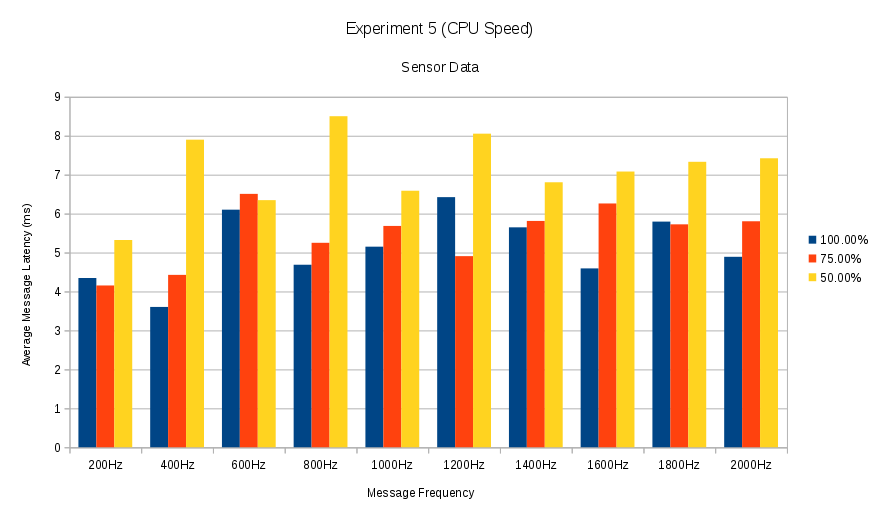
\includegraphics[width=\textwidth]{images/experiment5/sensor_data_all_freqs.png}
\caption{Experiment 5 - Sensor Data, All Frequencies}
\label{exp5-sensor-means-all-freq}
\end{figure}

\begin{figure}[H]
\centering
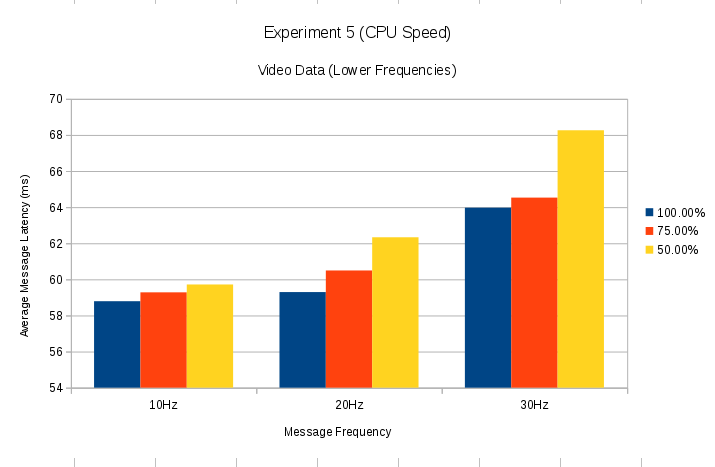
\includegraphics[width=\textwidth]{images/experiment5/video_data_low_freqs.png}
\caption{Experiment 5 - Video Data, Low Frequencies}
\label{exp5-video-means-low-freq}
\end{figure}

\begin{figure}[H]
\centering
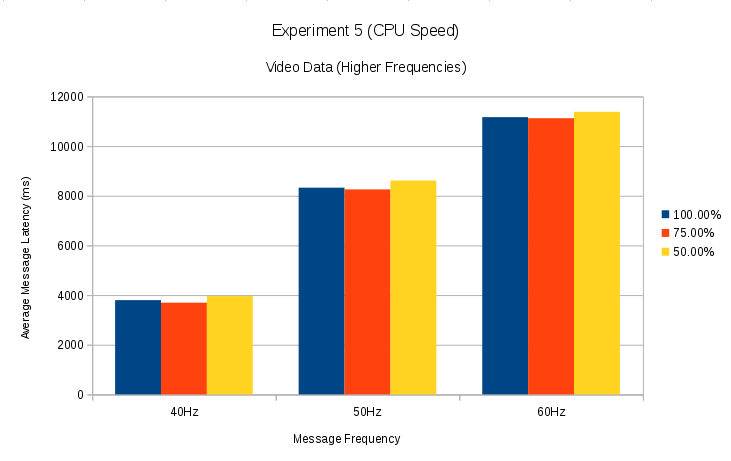
\includegraphics[width=\textwidth]{images/experiment5/video_data_higher_freqs.png}
\caption{Experiment 5 - Video Data, High Frequencies}
\label{exp5-video-means-high-freq}
\end{figure}

\end{document}
